\section{Generatory liczb równomiernych}
	\begin{frame}{Generatory liczb równomiernych}


	\textbf{14.3.1 Ogólne}
	\[
	x_{n+1}=f(\underbrace{x_{n},x_{n-1},\ldots,x_{n-k+1}}_{k \:stalych\: poczatkowych}) (mod\ \ M)
	\]
	Zal:
	$$
	D(f)=Z_{M}=\{0,\ 1,\ .\ .\ .\ ,\ M-1\}
	$$
	$$
	D^{-1}(f)=Z_{M}
	$$
	Takie generatory są {\it okresowymi}:
	\begin{center}
	$\exists N, K:\forall n\geq N x_{n}=x_{n}+jk$ , $j=1$, 2, . . .
	\end{center}
	$r$ -najmniejsza $N$:
    \begin{center}
	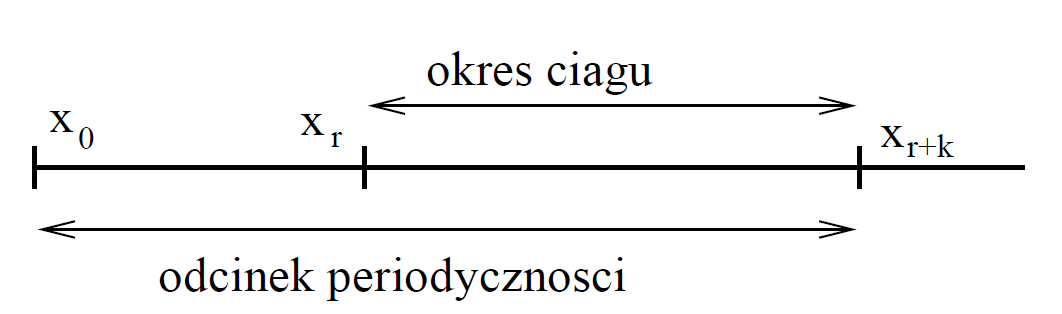
\includegraphics[width=70mm,height=20mm]{img/14/14_3_1_img}
	\end{center}
	\end{frame}

    \begin{frame}{Generatory liczb równomiernych}

	\textbf{14.3.2 Generator Fibonacciego}
	\begin{center}
 	$$x_{n+1} = (x_{n} + x_{n-1})(mod M)$$
	\end{center}
	- okres $\leq M^{2},$

	- prosty,

	- wada: korelacje w ciqgach generowanych liczb.
    \newline
	\end{frame}
    \begin{frame}
	\textbf{14.3.3 Generatory liniowe kongruentne}

	Większość generatorów to generatory {\it liniowe kongruentne}:\\ (1943, D.H. Lehmer)
	\begin{center}
 	$$I_{j+1} = (aI_{j}+c) mod\ m$$
	\end{center}
	gdzie:

    \[
    {\begin{rcases*}
	a - multiplier\\
	c - increment\\
	m - modulus
    \end{rcases*} liczby\ \ całkowite \ \ \in [0,m]}
    \]
	\end{frame}
    \begin{frame}
	Liczby zmiennoprzecinkowe: $\displaystyle \frac{I_{j+1}}{m}\in[0$, 1)
    \newline

	sekwencja: $I_{1}, I_{2}, I_{3}$, . . . ; $0\leq I_{i}\leq m-1$
    \newline \newline
    okres $\leq m$ ; zależy od wyboru $a, c \left\{\begin{array}{l}
	c\neq 0\ \rightarrow\ mieszane,\\
	c=0\ \rightarrow multiplikatywne.
	\end{array}\right.$

	Zaleta:

	a) {\it szybkość generacji}
	\newline

	Wady:

	a) {\it korelacje sekwencji}

	- $k$ -liczb losowych $\rightarrow$punkt w przestrzeni $k-D,$

	- punkty nie zapełniają równomiernie przestrzeni lecz układają się na $(k-1)-D$ 				hiperpłaszczyznach. Ilość płaszczyzn $\neq m^{\frac{1}{k}}, np. \ \ k=3, m=2^{32}\rightarrow 1600$ 		płaszczyzn

    \end{frame}
    \begin{frame}
	Kiedyś IBM wsławił się zdaniem ``{\it gwarantuje tylko losowość każdej liczby indywidualnie }''
    \newline
    \newline
	b) {\it niższe bity są} ``{\it mniej losowe}'' niż {\it wyższe}:

    - nie wykorzystywać liczb losowych w {\it kawałkach},

	- np. do generowania liczb losowych $\in[1, 10 ]$

	używać:

	$J=1+INT(10.0*$RANF (iseed) $)$

	a nie:

	$J=1+MOD(INT(100000.0*RANF($iseed)$),\ 10)$
    \end{frame}
